
\subsection{Axial Shielding Factor Measurements}

In these measurements, a witness cylinder was used as a magnetic
shield.  Small changes in the axial shielding factor are interpreted
as a change in the effective $\mu$ of the material.  This technique is
quite different than the usual mutual inductance techniques used by
other groups.  Our hope was that this geometry would give us more
confidence that the properties we were measuring were indeed related
to magnetic shielding properties rather than inherent properties of
the material.

\subsubsection{Magnetic Field Generation}

In order to measure the magnetic shielding factor, the witness
cylinder was placed within a homogeneous AC magnetic field.  The field
was created within the magnetically shielded volume of the prototype
magnetic shielding system (described previously in
Section~\ref{sec:previousmeasurement} in order to reduce unrelated magnetic noise
which might affect the measurement.  A solenoid inside the shielding
system was used to produce the magnetic field.  The radius and the
half length of the solenoid is 17.44~cm while the radius and the half
length of our innermost prototype passive shield is 18.44~cm.  In this
design, the field produced by the solenoid plus innermost shield
approximates an infinite solenoid producing a homogeneous magnetic
field internally.  The $\mu$ dependence of the reaction factor is
known to be considerably smaller than the $\mu$ dependence of the
axial magnetic shielding factor, hence any change in the fluxgate
amplitude with temperature can be ascribed to changes of the witness
cylinder, rather than changes in the innermost magnetic shield.

The solenoid has 14 turns with 2.6~cm spacing between the wires.  The
magnetic field generated by the solenoid was typically 1~$\mu$T.  The
solenoid current was varied sinusoidally at typically 0.01 to 10~Hz.

% Need to explain ``local coil'' as well, right here, right now.
% or just below, when Fig. geometry is shown.

\subsubsection{Witness cylinder and fluxgate magnetometer}

The witness cylinder was placed into this magnetic field generation
system as shown schematically in Fig.~\ref{fig:geometry}.  The
cylinder was held in place by a wooden stand.

A Bartington fluxgate magnetometer Mag-03IEL70 (low noise) measured the
magnetic field at the center of the witness cylinder. A plastic rod with 2.5~cm diameter used to hold the fluxgate flying lead. A hole with a diameter of 0.8~cm was drilled along the axis of the plastic holder to the middle. The fluxgate flying lead was then held at the center of the holder while a plastic screw prevented its movement. The plastic rod was then placed along the axis of symmetry of the witness cylinder and coupled to it by using two plastic end caps that screwed to the plastic rod.
In all data acquisitions, only one fluxgate flying lead was used.


% Taraneh: describe mounting fixture?  Explain that only one axis was
% used.
% plastic holder... (done)

%% while the
%%temperature of the shield was measured.


To increase the resolution of the measured signal from the fluxgate, a
Bartington Signal Conditioning Unit (SCU) with a low-pass filter set
to typically 10-100~Hz and a gain set to typically $>50$ was used.
The signal from the SCU was demodulated by an SRS830 lock-in amplifier
providing the in-phase and out-of-phase components of the signal.
(The sinusoidal output of the lock-in amplifier reference output
itself was normally used to drive the solenoid generating the magnetic
field.)  The time constant on the lock-in was typically set to 3
seconds with 12~dB filter.

\begin{figure}[h!]
\begin{center}
   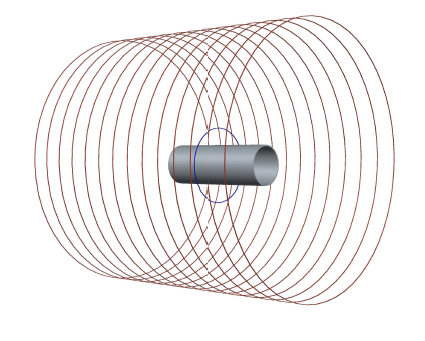
\includegraphics[width=0.8\textwidth]{geometry.PNG}
    \caption{Axial shielding factor measurement setup. The witness
      cylinder with a radius of 2.54~cm and a length of 15.2~cm is placed
      inside a solenoid with a radius and a half length of
      17.44~cm. The axis of symmetry is along the $z$-axis. The
      windings of the solenoid is shown in red. The blue coil with one
      turn is coupled to the witness cylinder and it has a radius of
      5~cm.  }
% Note to Jeff (self): fix this figure caption!!!
% (Need to look at it in the pdf form to think more about it.)
    \label{fig:geometry}
    \end{center}
\end{figure}

% Need to explain the local coil here, alternately, or above.



\subsubsection{Temperature measurement and data acquisition}


To reduce any potential magnetic contamination, T-type thermocouples
were used, which have copper and constantan conductors.  (K-type
thermocouples are magnetic.)


% To do (Taraneh and/or Jeff): where is the desciption of the
% temperature sensors!?!?!?  General data acquisition scheme?  How was
% the temperature even varied?  There are some serious missing pieces
% to the description of how the experiment was done!

% Note to Jeff: Done experiment description (for now - I expect some
% of the above is a part of what was discovered to be missing in
% writing the systematic errors section -- I will hope to fix it
% later).



\subsubsection{Data and Interpretation}

An example of the typical data acquired is shown in
Fig.~\ref{fig:B_vs_Temp}.  The field amplitude produced by the
solenoid was 2.6~$\mu$T, at a frequency of 1~Hz.
Fig.~\ref{fig:B_vs_Temp}(a) shows the temperature of the witness
cylinder over a four-day measurement.  The temperature changes are
about 3.5~K and are caused by temperature variations of the
laboratory.
% The following statement belongs more in the systematic errors section:
%
% For $f\lesssim 1$~Hz most of the measured fluxgate signal is in the
% in-phase component.
%
The magnetic field $B$ is anti-correlated with the temperature trend
in an shown in Fig.~\ref{fig:B_vs_Temp}(b).  Here, $B$ is the sum, in
quadrature, of the amplitudes of the in-phase and out-of-phase
components.  Magnetic field is then interpreted to depend on the
temperature, and they are graphed as a function of one another in
Fig.~\ref{fig:B_vs_Temp}(c).  The slope of Fig.~\ref{fig:B_vs_Temp}(c)
has been calculated using a linear fit to the data.  In this
measurement, the slope is found to be
$\frac{1}{|B|}\frac{d|B|}{dT}\simeq -1.5\%$/K.

Deviations from the linear straight-line dependence can be seen in the
data.  For example at the start of the data-taking, the slope is
almost zero.  This is typical of the data that we acquired, that the
magnetic field as a function of temperature would not necessarily lie
along a straight line, but rather would have different slope
temporarily after changing the direction of the temperature increase
or decrease.

A comprehensive set of systematic studies of the factors affecting the
slope were performed, and these are presented in
Section~\ref{sec:axialsyst}.  Based on these studies, we expect the
change in slope is either due to some properties of the material or
due to an unknown systematic error such as a long-time mechanical
relaxation of some element of the apparatus.

To express this inherent uncertainty in the slope, we phrase our
result as a range of slopes that were typical of data acquired over
time periods of $\sim$ days.  In general, we measured
0.3\%/K~$<\vert\frac{1}{B}\frac{dB}{dT}\vert<$~2.3\%/K with the sign
being negative.  The range also encompasses the typical deviation from
a linear $B(T)$ in the data (for example, those seen in
Fig.~\ref{fig:B_vs_Temp}(c).).  Since the data cannot be embodied by a
single temperature slope, the experiment tends to set a scale and sign
for the possible temperature dependence, rather than a value.

\begin{figure}[h!]
\begin{center}
   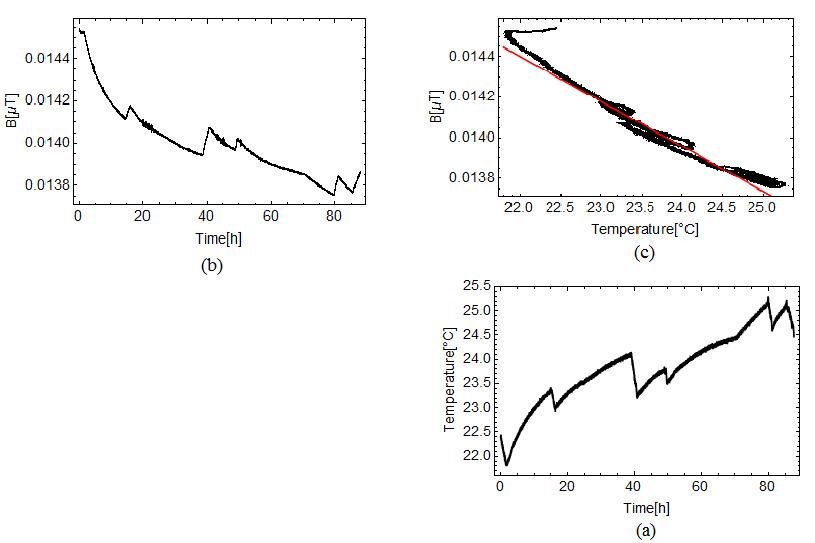
\includegraphics[width=0.5\textwidth]{B_vs_T.png}
    \caption{Ambient temperature and shielded magnetic field
      amplitude, measured over a 90 hour period. (a) temperature of
      the witness cylinder as a function of time.  (b) magnetic field
      amplitude measured by fluxgate at center of witness cylinder
      versus time.  (c) magnetic field versus temperature. The red
      line in (c) is a linear fit to data. At 22$^\circ$C,
      $\frac{1}{|B|}\frac{d|B|}{dT}=-1.5\%$/K.}
    \label{fig:B_vs_Temp}
    \end{center}
\end{figure} 


\subsubsection{Systematic Studies\label{sec:axialsyst}}

\paragraph{Methods of Temperature Variation}

In addition to ambient temperature changes, we tried other methods of
forced temperature change.  In one design, Tygon tubing was wrapped
around the witness cylinder in a spiral pattern to flow water whose
temperature could be controlled.  Mechanical stability issues clearly
dominated the systematic uncertainty in that measurement.  When water
was flowing, the flexibility of the tubing caused a movement in the
witness cylinder.  The motion was itself temperature-dependent because
warmer water caused the tubing to become more supple.  To address this
effect, the tubes were replaced by copper tubing.  But in this case,
the challenge was to create enough contact between the tubes and the
witness cylinder which was not successful. In another design, a TEC
was replaced with the tubing. The main issue with this design was that
it did not provide enough cooling for the witness cylinder and also it
was creating only local temperature changes on the witness
cylinder. In addition, despite of using heat sinks, the heat created
by the TEC itself made it very inefficient.  We also tried using
forced air to heat the witness cylinder.  This worked rather well, but
the heating had to be done slowly in order to avoid temperature
gradients across the apparatus, including the witness cylinder.  In
the end, using the ambient temperature changes in the room gave the
most reproducible results.  These followed a relatively stable diurnal
cycle with the function of the building's air conditioning system.

The changes in the $B$ vs.~temperature slope always correlate with
sharper changes in the temperature with time.  The effect is most
pronounced when a temperature that is decreasing with time suddenly
changes to increasing, or vice-versa.  However, we have incorporated
the uncertainty from this effect into our stated uncertainty already.


%\paragraph{Final Design} 

% This has all been said and could be deleted, I think:

%final design
%The final design included the witness cylinder, which was placed with
%a holder inside the innermost prototype passive shield. The
%temperature variations of the witness cylinder was due to the
%temperature changes in the room which was following the on and off
%cycles of the building air conditioner.
%A Bartington magnetic field
%sensor (fluxgate) was hold inside the witness cylinder at the centre
%by plastic holder. The signal from the sensor was then demodulated by
%an SRS830 lock-in amplifier. To convert the final measured voltage
%from the sensor to $\mu$T, the sum in quadratures of the in-phase and
%out of phase components of the lock-in amplifier was multiplied by the
%scaling factor on the magnetic field sensor which is 7 $\mu$T/V.


%%%%%%%%%%%%%%%%%%%%%%%%%%%%%%%%%%%%%%%%%%%%%%%%%%%%%%%%%%%%%%%%%%%%%%
% This is all new and needs to move up to the apparatus section:
%%%%%%%%%%%%%%%%%%%%%%%%%%%%%%%%%%%%%%%%%%%%%%%%%%%%%%%%%%%%%%%%%%%%%%
% The
% mu-metal alloy has a thermal conductivity of 0.35
% W/(cm$\cdot$K). Therefore, four thermocouples placed on different
% spots on the witness cylinder to correct for small temperature
% differences on each end of the witness cylinder.  In these
% measurements, the farther side of the passive shields had the end caps
% while the other side was left open to give access to the interior
% region. Based on the magnetic field maps inside the passive shields,
% for 10 $\mu$T applied magnetic field, the stability of the field was
% to 0.1 $\mu$T level and the magnetic field was even more stable closer
% to the closed side of the passive shields. Therefore the witness
% cylinder was pushed to the side with the end caps on the passive
% shields.
%%%%%%%%%%%%%%%%%%%%%%%%%%%%%%%%%%%%%%%%%%%%%%%%%%%%%%%%%%%%%%%%%%%%%%

% Another list
% - amplitude measurement on oscilloscope (no lock-in). (done)
% - speed of temperature change? temperature homogeneity?  (not here yet) 
% - other methods of cooling and why they didn't work. (not here yet)(done)
% - magnetic contamination by thermocouples (done)

% The above list maybe explains other possible variations on the
% method that you tried that all seemed to have worse systematic
% errors.

% Then, a list of systematic errors once you settled on the final
% measurement technique...

% - field profile/homogeneity (done)
% - mechanical stability (done)
% - thermal expansion (done)
% - temperature dependence of fluxgate and SCU (done)
% - temperature dependence of lock-in (done)
% - temperature dependence of coil resistance (not here yet) (done)
%    - Cupron/etc. study. plus
%    - measuring across the precision resistor
% - null measurement (Cu, and why it doesn't give the whole story, not here yet) (done)
% - effect of endcaps? (influence of external fields, not here yet)(done)
% - temperature dependence of reaction factor (negligible, not here yet)(done)
% - degaussing (not here yet)(done)
% - measurements on different witness cylinders? (not here yet)(done)
% - vibrations of the building?(done)
% - ...
%
% Another list is on the oldelog somewhere.  Please find it.
% The above list is longer and inclusive of the old list.
% See oldelog entry 141 in Magnetic Fields.
%
% This list of systematics is addressed now...

\paragraph{Field profile dependence and mechanical stability}

% Jeff got to here:  A concern in the measurement was that 

To eliminate the coupling of the field profile and mechanical
stabilities, another coil was used which was coupled to the witness
cylinder as shown in Fig.~\ref{fig:geometry}.  This also enabled us to
study the dependence of the field profile to $\mu(T)$. The result of
this study did not show a significant change and data was similar to
Fig. \ref{fig:B_vs_Temp} (c). Therefore, the systematic error due to
the field profile is smaller than the unknown systematic errors of
Fig. \ref{fig:B_vs_Temp} and similar figures.
% What is the value of the systematic error deduced from this study?
% I would say that the result of this study was that we got similar
% data to Fig. 3(c).  Therefore the systematic error due to field
% profile is smaller than the unknown systematic error of Fig. 3(c)
% and similar figures.  also partly addresses possible changes in
% reaction factor with temperature. (done)


%Temperature dependence of fluxgate and SCU
In these measurements, a Mag-03IEL70 Bartington magnetic field sensor which has individual sensor elements and a Mag-03SCU signal conditioning unit were used.
The magnetic field sensor is a low noise sensor with a range of $\pm$70 $\mu$T and it has a scaling temperature coefficient of 15 ppm/K.


As another mechanical stability study, the movement of the Bartington
fluxgate flying lead due to thermal expansion was estimated. If the
fluxgate flying lead move about 1 mm normal to its axis of symmetry
which is parallel to the axis of the witness cylinder, the magnetic
field will change about 30~ppm/K over 20~K temperature changes.  The
thermal expansion of the mu-metal cylinder is at the order of
10~ppm/K~\cite{kruppvdm}.  An SRS830 lock-in amplifier has 50
ppm/K amplitude stability. It is documented in the operating
manual \cite{bib:lockin}.

%We did this for the transformer technique
The temperature dependence of the coil resistance was also measured by
measuring the voltage across a temperature controlled 1~$\Omega$
resistor.
To address this effect, another measurement conducted with local coil with Cupron wire windings. Cupron has higher resistivity compared to copper wires. The results showed no linear correlation between the measured magnetic field and the temperature of the witness cylinder.
%The results?

%Taraneh: I calculated from the long summary
The stability of the system was tested by replacing the mu-metal
witness cylinder with a similar copper cylinder. For all those
measurements the stability was $<0.1$\%/K. Although these type of
measurements help to find an error bar on the stability of the system
in general, they do not help to find the sources of the systematic
uncertainty.


%effect of the end caps
In this experiment, one side of our prototype passive shield was
closed with the end caps while the other side left open for easier
access to the interior region. The result of the magnetic field map
inside the prototype shield when the solenoid was turned on showed
that closer to the far side of the shield, where the shield is closed,
the magnetic field is more uniform. For a 10$\mu$T applied magnetic
field the maximum change of the magnetic field along the axis of the
passive shield was the order of 0.1~$\mu$T.  Therefore the witness
cylinder was pushed to the far side of the prototype shield to reduce
the non uniformity of the magnetic field.
%This is from oldElog entry 146: field map by Andrew Harrison

%temperature dependence of reaction factor
The changes in magnetic permeability has an effect on the measured
magnetic field inside the witness cylinder. Since the reaction factor
for this geometry is not strongly correlated to $/mu$ in
Fig. \ref{fig:Magnetic_Field}, the changes of the magnetic field due
to magnetic permeability changes in negligible. For XXX change in
$\mu$ the magnetic field internal to the witness cylinder changes by
XXX.

%degaussing
The magnetization of the prototype passive shield changes the magnetic
permeability of the material and so the reaction factor changes. The
degaussing procedure has a considerable effect on the initial magnetic
field.
%what next?

%different witness cylinders
Three witness cylinders were tested for these measurements. In most
cases, despite keeping the conditions the same, the results were
significantly different for each witness cylinder. The systematic
studies could not address these sources of error. As a result these
changes is believed to be driven by the intrinsic properties of the
witness cylinders.  In general, annealing process and take-out
temperatures have a strong effect on the properties of the shields and
so their $\mu$ value.
%vibration
Since the experiment site is located at the heart of downtown it is
also possible that vibrations of the building affected the experiment
setup and its machanical stability.

Although for most of the measurements the general trend of $B(T)$
graphs was consistent, the shape and positions of the nonlinear parts
of $B-T$ graphs were changing.


% Two possibilities:

% 1. unknown systematic error(s)

% 2. complicated material properties that don't follow a straight line
% could depend on material history themselves.

% Therefore we state a range which should be indicative of the scale
% of possible temperature dependence.


\subsubsection{Geometry correction and determination of $\mu(T)$}

To relate the data to $\mu(T)$, the shielding factor of the witness
cylinder as a function of $\mu$ must be known.  Finite element
simulations in FEMM and OPERA were performed to determine this factor.

Combining the measurement and the simulations, the temperature
dependence of the effective $\mu$ (at $\mu$=20000) can be calculated
by
\begin{equation}
\frac{1}{\mu}\frac{d\mu}{dT}=-\frac{\frac{1}{B}\frac{dB}{dT}}{\frac{\mu}{B}\frac{dB}{d\mu}}.
\end{equation}

From the simulations the ratio $\frac{\mu}{B} \frac{dB}{d\mu}$ was
calculated.  A linear model of the material was used where
$\bold{B}=\mu \bold{H}$ and $\mu$ is a constant independent of
$\bold{H}$.  The term $\frac{\mu}{B}\frac{dB}{d\mu}\neq 1$ because the
witness cylinders are open ended, and hence even for very large
$\mu\rightarrow\infty$ the shielding factor asymptotically approaches
a constant rather than infinity.

The simulations differed slightly in their results, dependent on
whether OPERA or FEMM was used, and whether the solenoidal coil or
loop coil were used.

Based on the simulations, the result is
$\frac{\mu}{B}\frac{dB}{d\mu}=0.42-0.50$ for the solenoidal coil, with
the lower value being given by FEMM and the upper value being given by
a 3D OPERA simulation, for identical geometries.  This is somewhat
lower than the value suggested by
Paperno~\cite{bib:paperno-open-ended} in his fits to simulations
performed in OPERA, which we estimate to be 0.6.  For the loop coil,
we determine $\frac{\mu}{B}\frac{dB}{d\mu}=0.56-0.65$, the range being
given again by a difference between FEMM and OPERA.





Taking all these systematics into account, in this method it was found that 0.6\%/K
$\lesssim\frac{1}{\mu}\frac{d\mu}{dT}\lesssim 2.3\%$/K. 



%\begin{itemize}
%\item Describe experimental setup and important considerations
%  (e.g. relationship of data to effective $\mu$)
%\item Explain B, H, f, and dominant systematic effects.
%\item One figure of experimental setup?
%\item One data graph?
%\item State overall result and systematic error.
%\end{itemize}
